\documentclass{scrartcl}

\usepackage[ngerman]{babel}

\usepackage[utf8]{inputenc}
\usepackage{hyperref,xcolor,microtype,ifthen}
\usepackage{csquotes}

\usepackage{graphicx}
\usepackage{svg}

\usepackage{helvet}
\renewcommand{\familydefault}{\sfdefault}
\fontfamily{phv}\selectfont

\linespread{1.25}

\title{Mobile Application Lab}
\subtitle{Dokumentation}
\date{07.03.2018}
\author{Max Landthaler,Manuel Konstantin Hinke}

\begin{document}

\maketitle

\section{Einleitung}
\subsection{Motivation}


Im Rahmen des Anwendungsfaches Mobile Application Lab wurde eine Quartett App geschrieben. Ziel des ganzen war es einen grundlegenden Einstieg in die Android Programmierung zu finden. Da ein Spiel viele verschiedene Bereiche abdeckt eignet es sich ideal für den Lernprozess.
Übergeordnete Motivation war der Lernprozess wofür sich dieses Szenario sehr gut eignet.

\subsection{Ziel}

Das hiermit erklärte Ziel dieses Projekts ist die Entwicklung einer Quarett-App fortwährend auch Unicorn-Quartett genannt. Es sollen gängige und Vorgehensweisen und Best Practices erarbeitet werden.
Dabei ist auch Ziel herauszufinden welche Schwierigkeit es gibt beim Implementieren für Android Betriebsysteme unterschiedlicher Versionen zu entwickeln.


\subsection{Aufbau}

Die folgende Dokumentation beschreibt den Enwicklungs und Implementierungsablauf.
Dabei werden zuerst Grundlegende Rahmen definiert und eine Anforderungsanalyse erstellt, die sowohl funktionale als auch nicht funktionale Anforderungen erfüllt.
Auch das erdachte Design und Struktur Konzept wird beschrieben um auch eventuell vergleichen zu können wo sich das Endresultat mit dem tatsächlich erreichten unterscheidet.
Es folgen dann ausgewählte Implementierungsdetails und abschließend ein Abgleich der Anforderungen.

\section{Grundlagen}
\subsection{Quartettspiel}

Beim klassischen Quartett geht das darum, möglichst viele Quartette (Ansammlung von 4 Karten gleicher Kategorie) zu erspielen.
Dabei werden die Werte der Kontrahenten verglichen und der höhere Wert gewinnt. Der Gewinner bekommt die unterlegenden Karten.
Das Unicorn-Quartet spielt im Standardmodus eine Abwandlung des klassischen Quartetts, das sich Supertrumpf nennt bzw. im Umgangssprachlichen als
Autoquartett  bezeichnet wird. Es folgen die genauen Beschreibungen der Spielelemente und Spielmodi.
\subsubsection{Quartettkarte}

\begin{figure}[!ht]
\begin{center} 
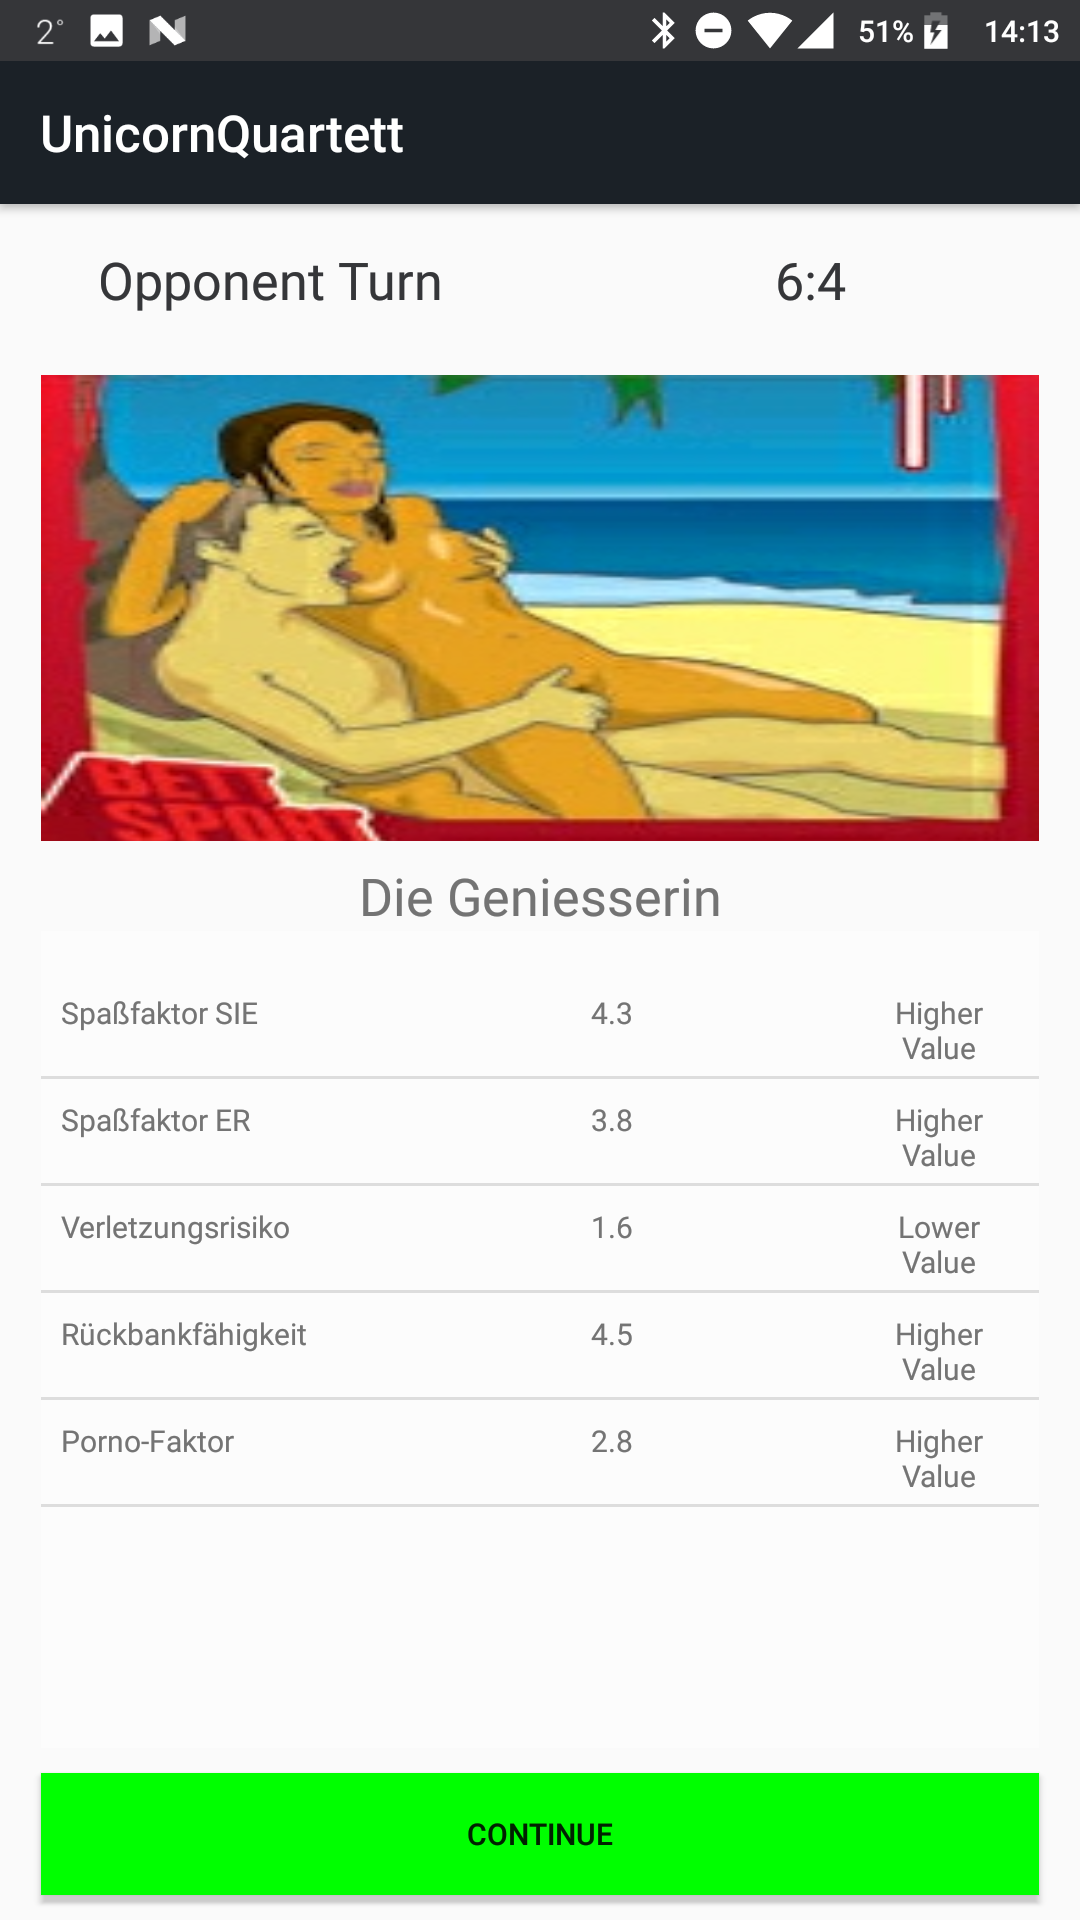
\includegraphics[scale=0.1]{pics/QuartettKarte.png}
    \caption{Die Geniesserin  aus dem Bettsport Deck}
\end{center}
\end{figure}

In Abb.1 wird eine Quartettkarte im Unicorn-Quartett visualisiert.
Ganz oben wird der aktuelle Spielstand angezeigt und wer aktuell am Zug ist.
Dann folgt ein Bild, auf dem das entsprechende Objekt der Karte zu sehen ist, in diesem Fall ein Auto.
Unten werden die zur Auswahl stehenden Werte angezeigt.


\subsubsection{Spielverlauf}
An einem Spiel nehmen der Spieler und eine Künstliche Intelligenz als Kontrahent teil.
Der menschliche Spieler legt ein Quartett und den Spielmodus fest.
Hierbei kann sich zwischen einem normalen Spiel und dem sog. Unicorn Modus entscheiden.
Zu Spielbeginn werden die Karten des Quartetts gemischt und gleichmäßig an die beiden Kontrahenten verteilt.
Der menschliche Spieler ist immer zuerst an der Reihe und wählt einen Wert von seiner aktuellen Karte aus, mit dem er seinen Kontrahenten stechen möchte.
Nachdem er seinen Wert bestätigt hat, werden sein Wert und der des Kontrahenten verglichen. Wer den besseren Wert hatte, bekommt die Karte des Verlierers.
Anschließend ist der andere Spieler an der Reihe, d.h. es wird unabhängig vom Ausgang der vorheringen Runde immer abgewechselt.
Gewinner des Spiels ist ganz klassisch der Spieler, der am Ende alle Karten hat.

Um etwas Abwechslung in den normalen Quartett Spielfluss zu schaffen, wurde der Unicorn Modus entwickelt.

\subsubsection{Spielmodi}

\textbf{Normal:}
Der klassische Modus. Hier wird abwechselnd gespielt. Gewonnen hat derjenige, der am Ende alle Karten hat.

\textbf{Unicorn}:
Der überraschende Modus. Auch hier wird abwechselnd gespielt. Jedoch können beide Kontrahenten ab einer Siegesserie von 3 hintereinander gewonnen Runden, sofern sie selbst
an der Reihe sind, besondere, zufällig generierte Aktionen ausführen, die zu ihrem direkten Vorteil sind.
Außerdem werden zufällig generierte Events, die beide Spieler positiv oder negativ beeinflussen, in das Spiel gestreut, ohne dass die Spieler darauf Einfluss nehmen können.
Gewonnen hat der Spieler, der alle Karten hat oder die richtige Aktion ausgespielt hat.


\subsection{Mobile Anwendungen}
Ziel dieses Projektes war es, sich mit der Entwicklung von mobilen Anwendungen auf einer beliebigen Plattform zu befassen und erste Erfahrungen zu sammeln.

Da beide Entwickler ein Android Endgerät besitzen und auch Interesse an dieser Umgebung haben, war sofort Android als Plattform gesetzt.
 
Weitere Vorteile bei der Entwicklung von Android Anwendungen sind die große Verbreitung von Android Endgeräten und die Verwandtheit zur normalen Java Entwicklung.

Im Hinblick auf mobile Anwendungen fallen besonders die beschränkten Ressourcen wie begrenzte Akkukapazität, Arbeitsspeicher, Rechenleistung und Festplattenspeicher ins Gewicht.
Im Vergleich zu normalen PCs oder Servern stehen auf einem mobilen Gerät viel weniger Ressourcen zur Verfügung, die zudem von vielen Anwendungen sowie dem System gleichzeitig verwendet werden.

\subsection{Libraries und Frameworks}
Um einige Funktionen der Applikation nicht selbst implementieren zu müssen
wurden folgende zusätzliche Programmbibliotheken und Frameworks verwendet:

\noindent
\textbf{Volley, https://github.com/google/volley} \newline
Volley ist eine Bibliothek, die es sich zur Aufgabe gemacht hat, Netzwerkoperationen sehr einfach und effektiv durchzführen.
Mithilfe von Volley wurde das Downloaden von neuen Decks und Karten realisiert.

\ \newline
\textbf{CircleImageView, https://github.com/hdodenhof/CircleImageView} \newline
Hiermit wird eine runde ImageView eingeführt, die für die Abbildung des Profil Bildes verwendet wurde.

\ \newline
\textbf{Realm, https://github.com/realm/realm-java} \newline
Realm ist eine objektorientiere Datenbank, die sich gerade für Android eignet, um einfach und ohne echte Datenbankbefehle tatsächliche Objekte in einer Datenbank zu verwalten, was die Behandlung der einzelnen Spielstatistiken und Decks sowie deren Karten, Attribute und Bilder sehr einfach gestaltet. 


\section{Anforderungsanalyse}
\subsection{Funktionale Anforderungen}

Ein wichtiges Thema im Vorfeld der Implementierung war es die Anforderungen an das Unicorn Quartett klar zu definieren.
Im folgenden werden die funktionalen und nicht funktionalen Anforderungen
aufgelistet, die vor der Entwicklung der Applikation formuliert wurden. 

\ \newline
\textbf{FA1 Ladebildschirm} \newline
Beim Öffnen der App erscheint ein Ladebildschirm, in dem das Logo der App dargestellt wird. Zudem befindet sieht der Nutzer eine Fortschrittsanzeige mit Statusmeldungen. Anschließend wird der Nutzer automatisch auf den Startbildschirm weitergeleitet.
\ \newline
\textbf{FA1-0 Nutzer erstellen} \newline
Wenn der Nutzer zum ersten Mal die App startet, wird er dazu aufgefordert, einen Benutzer zu erstellen. Dies muss zu beim Start der App getätigt werden. Zur Erstellung des Nutzer wird ein Name und ein Profilbild welches wahlweise mit der Kamera aufgenommern werden kann oder aus der Galerie ausgewählt werden kann, benötigt. Über den Namen kann der Nutzer von anderen Nutzern identifiziert werden.
\ \newline
\textbf{FA1-1 Startbildschirm} \newline
Auf dem Startbildschirm befinden sich 5 Elemente: Über Buttons mit entsprechenden Icons gelangt der Nutzer zu den folgenden Ansichten:
- Spielen
- Kartenverwaltung/Kartengallerie
- Freunde
- Rangliste
- Profil
\ \newline
\textbf{FA2-1 Spiel erstellen | Offline Spiel} \newline
Auf der Spielansicht kann der Nutzer zwischen  zwei Optionen wählen:
- Offline Spiel gegen die „KI“
- Online Spiel gegen Freunde
Nach der Auswahl gelangt der Spieler auf die Ansicht, in der er sich zwischen den verschiedenen Spielmodi entscheiden kann.
\ \newline
\textbf{FA2-2 Online Spiel} \newline
Wählt der Spieler die Option „online“ aus, kann er entweder gegen einen zufällig ausgewählten Online-Spieler spielen oder er wählt einen Spieler aus seiner Freundesliste aus.
\ \newline
\textbf{FA2-3 Spielmodi} \newline
Der Nutzer kann zwischen zwischen zwei Spielmodi auswählen:
- Standard (Stechen)
- Unicorn Mode (Stechen, aber mit globalen Events und Sonderkarten)
\ \newline
\textbf{FA2-4 Spiel} \newline
Im eigentlichen Spiel sieht der Spieler je Runde genau eine Karte mit aktuellem Bild und den Werten der Karte. Der Nutzer wählt einen Wert aus, der ihm am vielversprechendsten erscheint.
Dann erfolgt ein Wechsel der Anzeige von der einzelnen Karte des Spielers zu einer Gegenüberstellung der beiden Karten der gegeneinander antretenden Spieler. Der Wert des Siegers wird grün markiert, der des Verlierers rot. 
Der aktuelle Spielstand wird eingeblendet und die nächste Runde beginnt.
Dabei wird sichtbar visualisiert wer gerade am Zug ist.
\ \newline
\textbf{FA3-1 Kartenverwaltung} \newline
In der Kartenverwaltung wird dem Spieler eine Übersicht aller möglichen Decks angezeigt. Vorhandene Decks werden in Farbe abgebildet, Decks, die erst mit der Zeit erworben werden können, sind zu Beginn ausgegraut.
Klickt der Nutzer auf ein Deck, kann er sich die einzelnen Karten darin ansehen.
\ \newline\\
\textbf{FA4-1 Bestenliste} \newline
In der Bestenliste werden die Top 5 Online Spieler angezeigt.
\ \newline
\textbf{FA5-1 Freunde} \newline
In der Freundesübersicht kann der Nutzer entweder einen Freund über seinen Namen hinzufügen oder kann die Liste seiner Freunde ansehen, wenn diese die Freundschaftsanfragen angenommen haben.
\ \newline
\textbf{FA6-1 Spieler Profil} \newline
Im Spielerprofil kann der Nutzer seinen Account mit Google verknüpfen, um seinen Fortschritt auch online zu speichern und um online spielen zu können.
Außerdem kann er hier seine Spielhistorie einsehen.
\ \newline

\subsection{Nicht Funktionale Anforderungen}
\ \newline
\textbf{NFA1 Aktuelle Version der Betriebssysteme} \newline
Die Oberfläche der App sollte sich an aktuelle Designrichtlinien orientieren und auf den gängigsten Versionen lauffähig sein.
\ \newline

\textbf{NFA2 Usability Ziele} \newline
Die App sollte einfach und verständlich aufgebaut werden sodass sich der Nutzer intuitiv in den Menüs zurechtfinden kann.
\ \newline

\textbf{NFA3 Feedback} \newline
Die App sollte dem Nutzer unter bestimmten Bedingungen ein Feedback geben.
Der Nutzer darf nie im Unklaren darüber sein was die App gerade macht.

\pagebreak
\textbf{NFA4 Selbsterklärbarkeit} \newline
Die App sollte selbsterklärend aufgebaut sein. Der Nutzer sollte keine Probleme beim Verständnis der Funktionen oder Icons haben und ohne Hilfe das System bedienen können. Die App sollte ohne eine Anleitung bedienbar sein.
\ \newline

\textbf{NFA5 Benutzerfreundlichkeit} \newline
Die App sollte benutzerfreundlich aufgebaut sein, dass heißt der User soll einen positiven Eindruck von der App bekommen und sie gerne verwenden.
\ \newline

\textbf{NFA6 Verfügbarkeit} \newline
Die App sollte in den üblichen Smartphone Auflösungen darstellbar sein und sich auch an die Größenänderungen des Displays anpassen.
\ \newline
\\
\textbf{NFA7 Robustheit} \newline
Die App sollte gegenüber Fehleingaben robust sein.
\ \newline

\textbf{NFA8 Reaktionszeit} \newline
Die App soll innerhalb so kurzer Zeit reagieren, dass der Nutzer keine nennenswerte Wartezeiten abwarten muss, ohne zu wissen, was vor sich geht.
\ \newline

\textbf{NFA9 Statusrückmeldung} \newline
Wenn die App nicht innerhalb angenehmer Reaktionszeiten reagieren kann, soll der Nutzer über eine aussagekräftige Anzeige über den aktuellen Zustand der App informiert werden.
\ \newline



\section{Konzept und Entwurf}
\subsection{Mockups}
Im Vorfeld der Implementierung musste natürlich auch ein Entwurfskonzept erarbeitet werden. Dieses Entwurfskonzept sollte die grundlegende Architektur der Applikation beschreiben und die einzelenen Screens in einer schlichten und funktionalen Art vorbereiten.
Wir haben bei der Erstellung dieser Screens auf eine softwareunterstütze Lösung verzichtet und haben diese per Hand erstellt.
\begin{figure}[!ht]
\begin{center}
	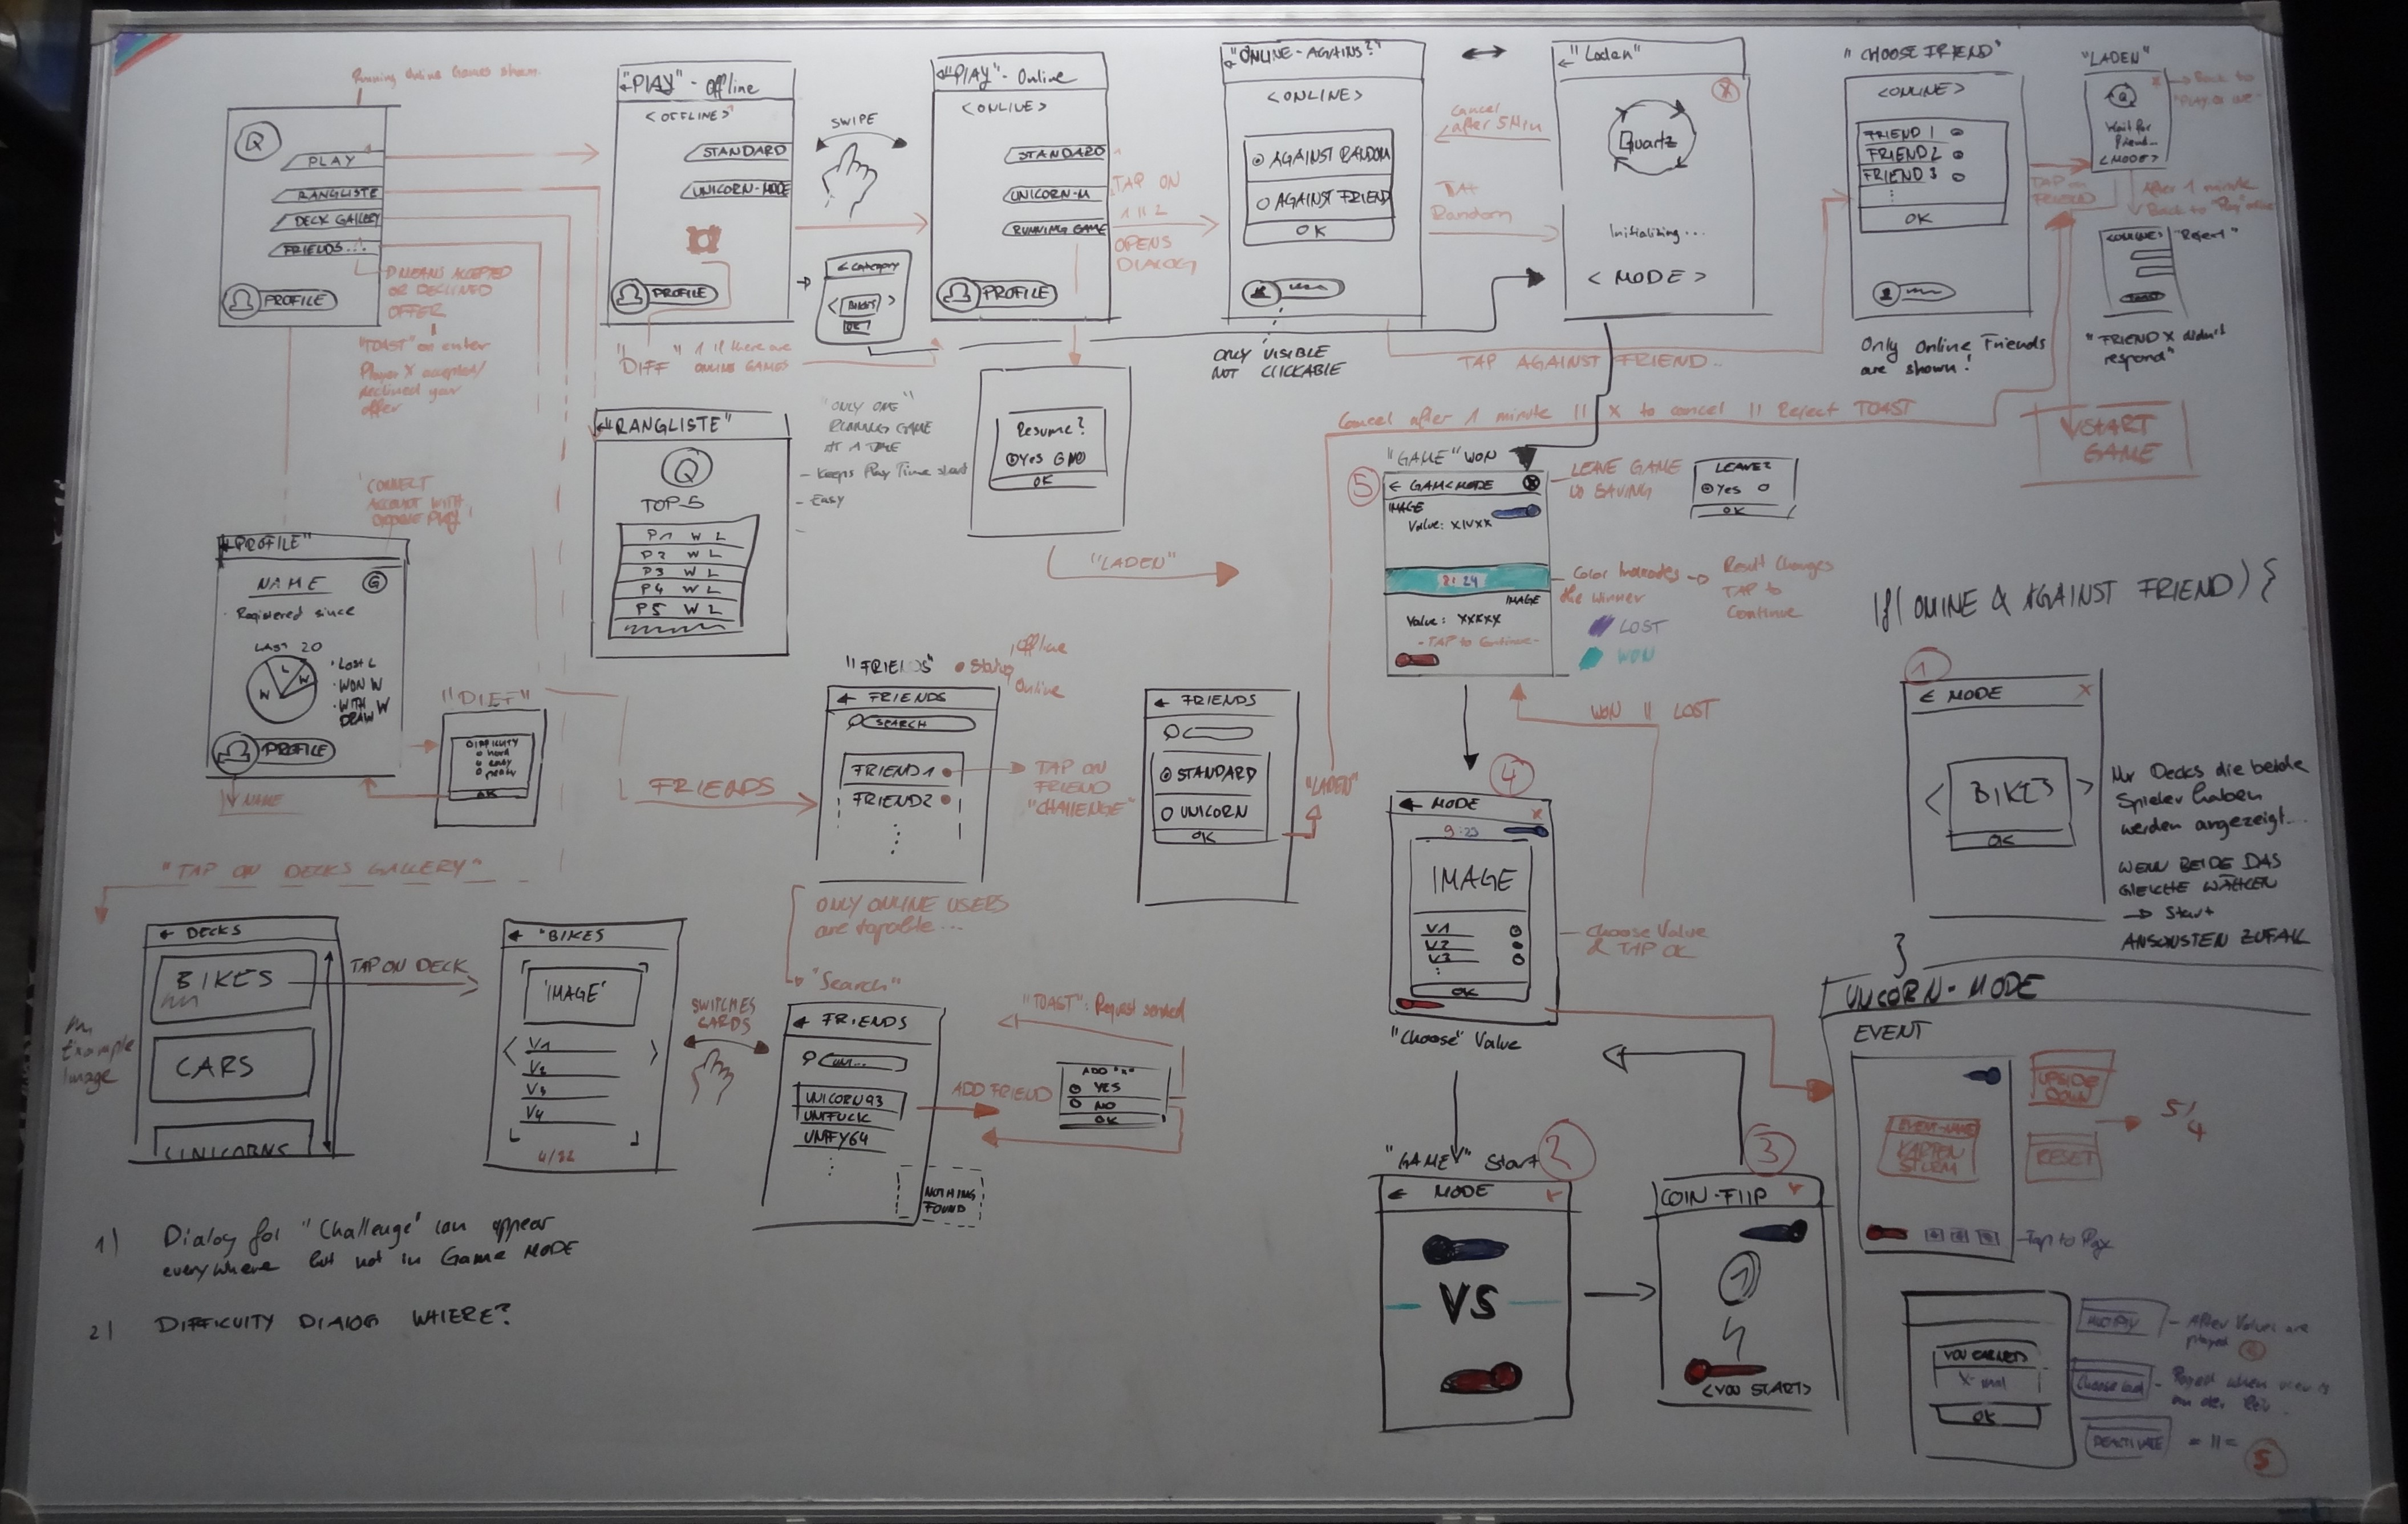
\includegraphics[scale=0.5]{pics/overview.png}
	\caption{Komplettansicht-Prozessablauf}
	\label{overview}
\end{center}
Darstellung der gesamten Möglichkeiten beziehungsweise Prozesse die in der App realisiert werden sollten. 
Das Profil ist von allen Screens aus erreichbar es sei denn man befindet sich in einem Spielprozess.
\end{figure}

\begin{figure}[!ht]
\begin{center}
	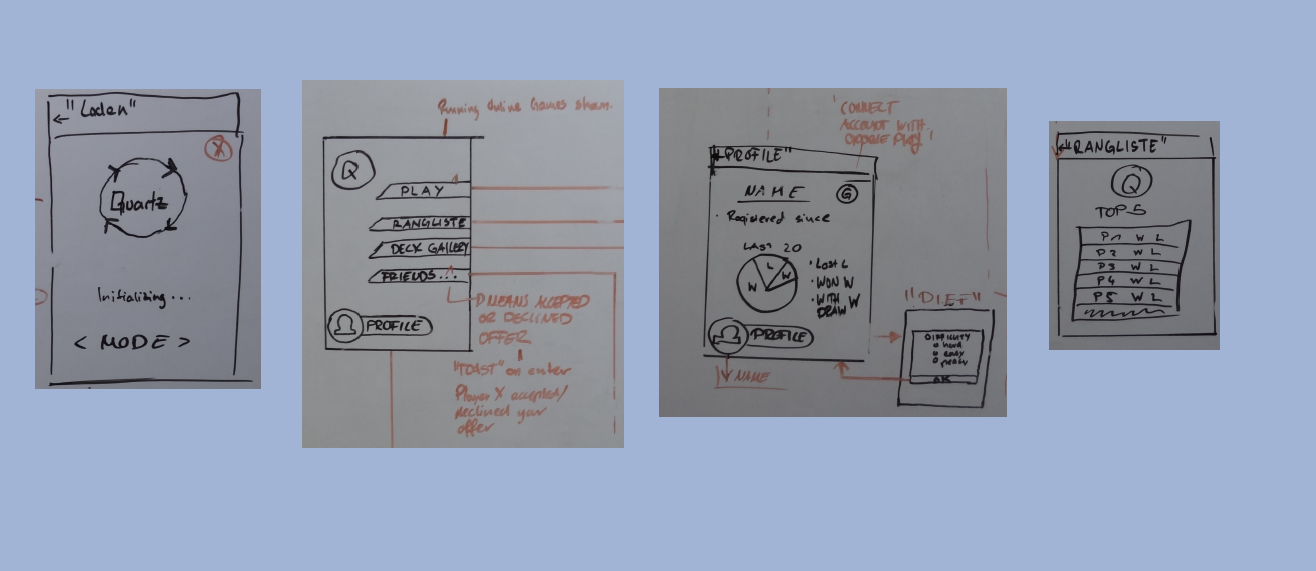
\includegraphics[scale=0.4]{pics/userhandling.png}
	\caption{Erstellung des Benutzers und bearbeiten der Daten}
	\label{UserProfil}
\end{center}
Abbildung ~\ref{UserProfil} skizziert den Prozess, welchen der Benutzer
vollführen muss, um einen Nutzer zu erstellen und wie er eingegebene Daten später wieder ändern kann.
\end{figure}

\begin{figure}[!ht]
\begin{center}
	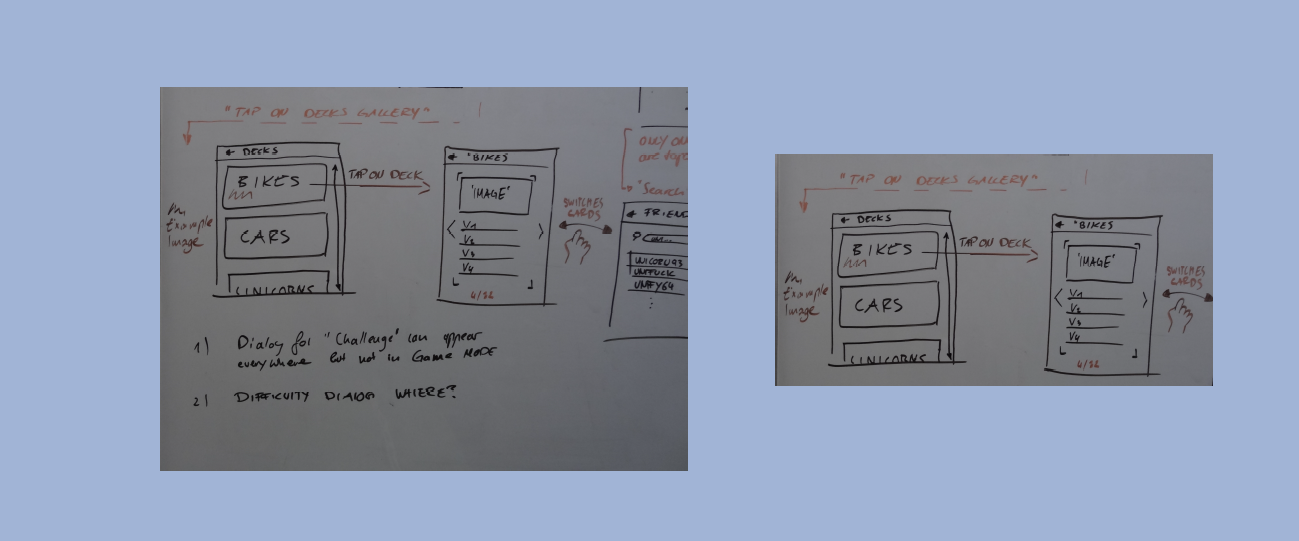
\includegraphics[scale=0.4]{pics/deckgallery.png}
	\caption{Kartenansicht/Kartengallerie}
	\label{DeckGallery}
\end{center}
In der Abbildung ~\ref{DeckGallery} wählt der Nutzer eines seiner Decks aus und kann sich dessen Karten ansehen.
\end{figure}

\begin{figure}[!ht]
\begin{center}
	\centering
	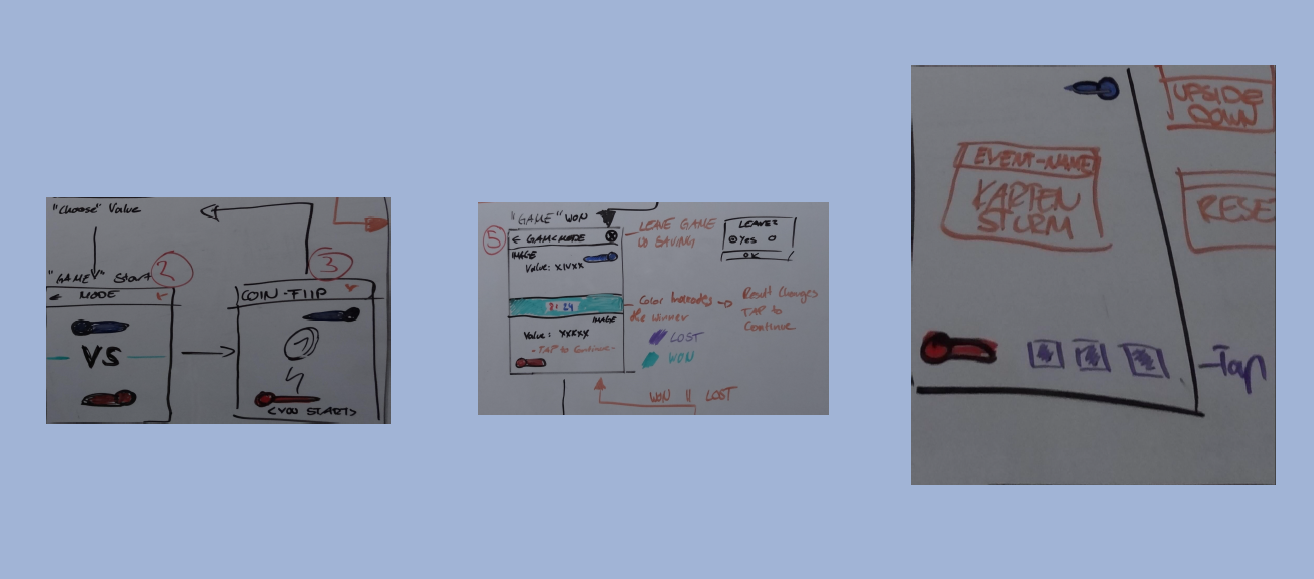
\includegraphics[scale=0.4]{pics/gameplay.png}
	\caption{Spielablauf}
	\label{gamePlay}
\end{center}
Diese Screens zeigen den grundlegenden Ablauf eines Spiel. Diese sind zwar unterschiedlich je nach Modi aber zum Zeitpunkt der Mockups ging es nur um ein generelles Darstellen des Prozesses.
~\ref{gamePlay} zeigt.
\end{figure}
\clearpage

\section{Implementierung}
\subsection{Ausgewählte Implementierungsdetails}
\subsubsection{Galerie}

\begin{figure}[!ht]
  \centering
  \begin{minipage}{0.45\textwidth}
    \centering
    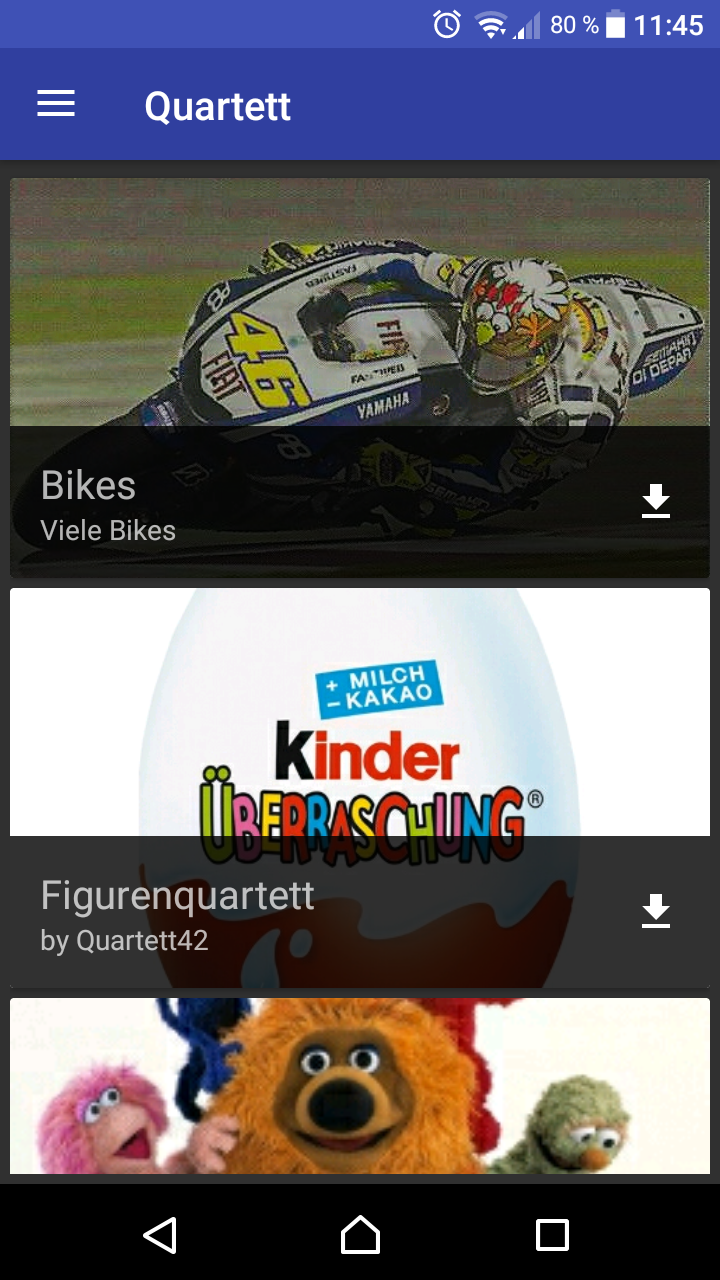
\includegraphics[width=4cm]{img/gallery_decks.png}
    \caption{Deckansicht}
  \end{minipage}
  \hfill
  \begin{minipage}{0.45\textwidth}
    \centering
    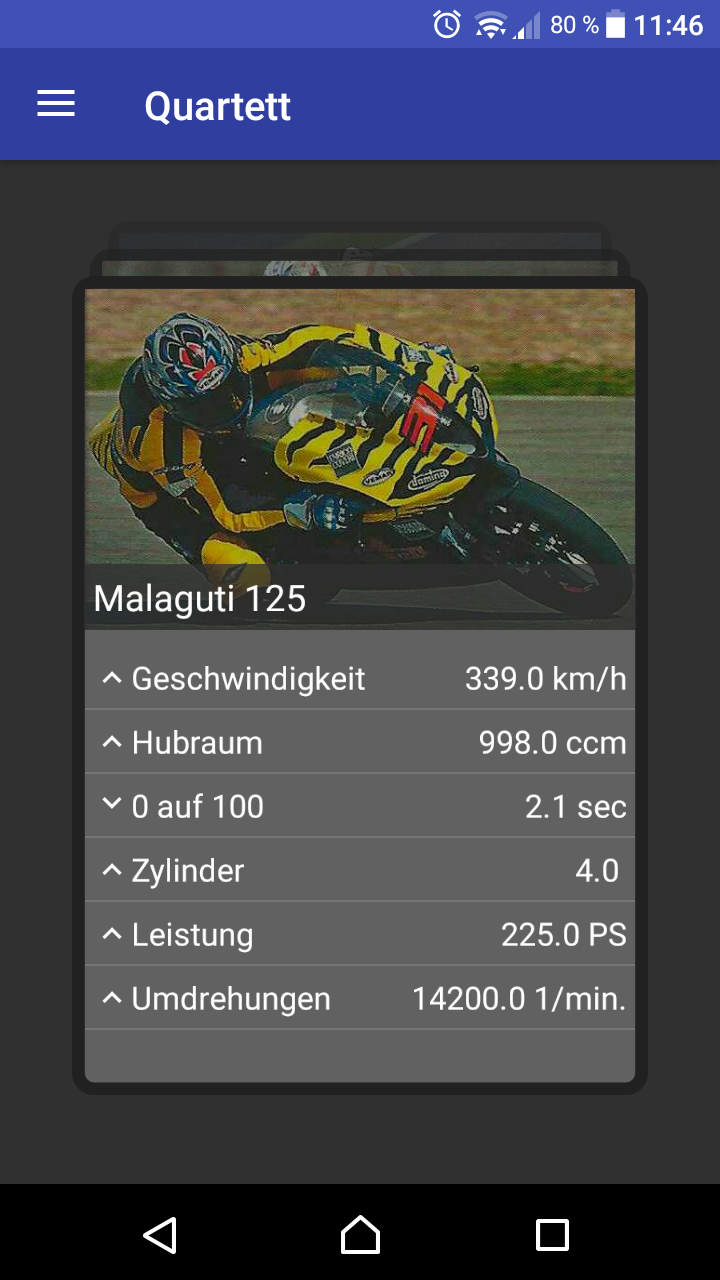
\includegraphics[width=4cm]{img/gallery_cards.png}
    \caption{Kartenansicht}
  \end{minipage}
\end{figure}

\noindent
In der Galerie werden alle Kartendecks aufgelistet, die auf dem Smartphone
vorhanden sind oder vom Server heruntergeladen werden können. Heruntergeladenen
Decks könne durch Antippen geöffnet werden. In der geöffneten Ansicht kann der
Benutzer durch vertikale Wischgesten durch die einzelnen Karten des virtuellen
Kartenstapels blättern. Tippt der Benutzer ein Deck an, welches nicht
heruntergeladen ist, wird ein Dialog geöffnet in welchem das Herunterladen des
Decks bestätigt oder abgelehnt werden kann. Das Deck wird nicht direkt geladen,
da sich der Benutzer eventuell in einer Netzwerkumgebung befindet, in welcher
durch Downloads Kosten entstehen können. Durch den Bestätigungsdialog wird dem
Benutzer somit eine Möglichkeit gegeben den Download zu einem späteren Zeitpunkt
mit günstigeren Netzwerkbedingungen zu starten. Wird der Dialog bestätigt startet
der Download des Decks. Im Listenelement des Decks wird ein Ladebalken angezeigt
und im Notification Drawer wird eine Notification erstellt die ebenfalls den
Fortschritt des Downloads anzeigt. Nach erfolgreichem Download wird die
Notification geschlossen und der Ladebalken verschwindet wieder. Das Deck ist
dann persistent auf dem Gerät gespeichert und kann nun auch ohne
Internetverbinung angezeigt werden. Zudem können nun auch die Karten des Decks,
wie oben beschreiben angezeigt werden. Auch kann das Deck nun im Einzelspieler
Modus verwendet werden.

\begin{figure}[!ht]
  \centering
  \begin{minipage}{0.45\textwidth}
    \centering
    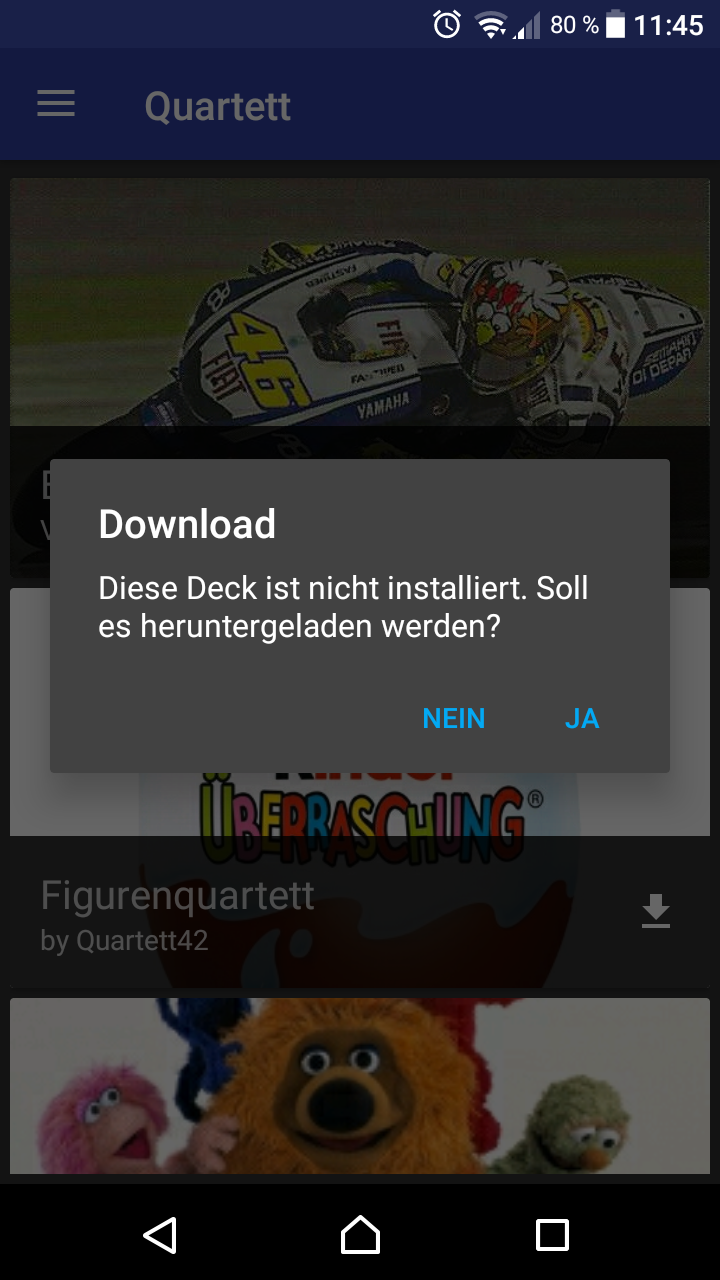
\includegraphics[width=4cm]{img/gallery_dialog.png}
    \caption{Download-Dialog}
  \end{minipage}
  \hfill
  \begin{minipage}{0.45\textwidth}
    \centering
    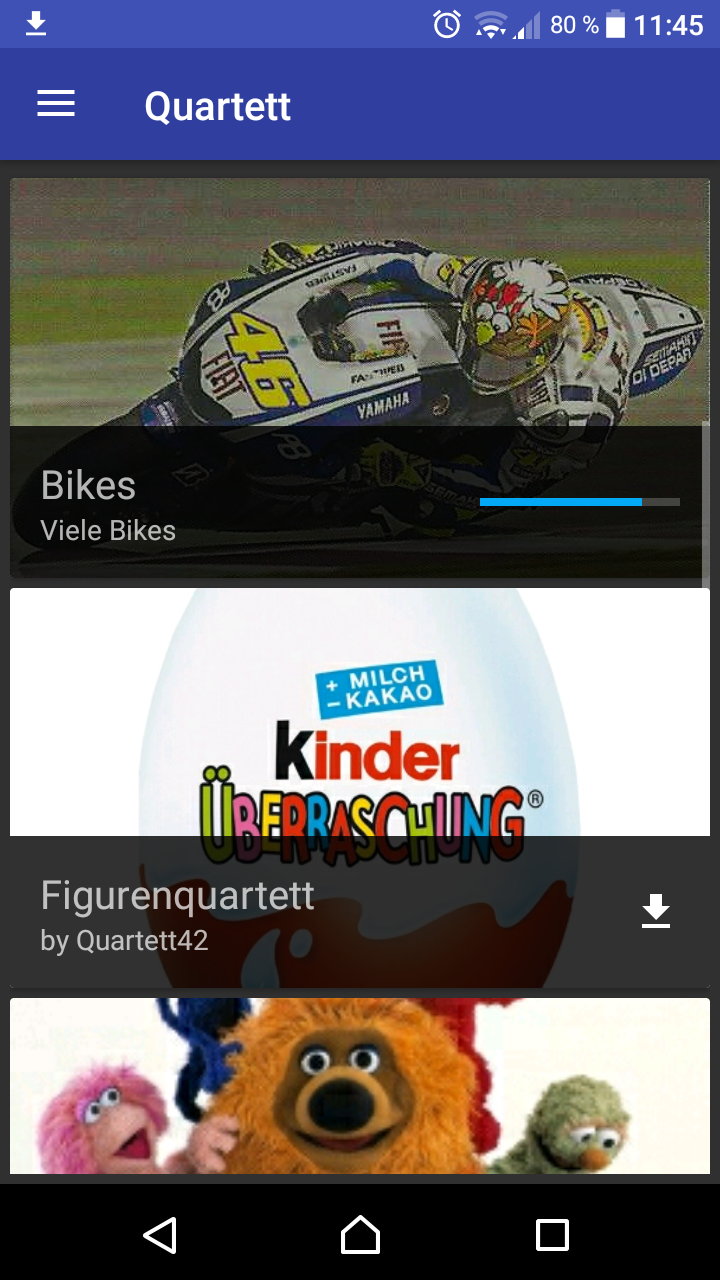
\includegraphics[width=4cm]{img/gallery_download.png}
    \caption{Download-Fortschritt}
  \end{minipage}
\end{figure}

\ \newline
Um die Galerie mit diesen beschriebenen Funktionen zu realisieren, waren einige
besondere Implementierungsmethoden notwendig. Da den meisten Decks und Karten
relativ hochauflösende Bilder zugeordnet sind, entstehen beim Anzeigen der Decks
bzw. Karten Verzögerungen, da große Datenmengen geladen werden müssen. Dabei ist
außerdem zu erwähnen, dass das Laden der Bilder der Decks, die nicht auf dem
Gerät gespeichert sind, über das Netzwerk erfolgt und somit zusätzliche
Verzögerungen entstehen. All diese Verzögerungen sind als starke Ruckler
bemerkbar und beinträchtigen das Nutzererlebnis erheblich. Das Laden der Bilder
wurde daher auf einen zweiten Thread ausgelagert. Somit kann der Benutzer
weitere Interaktion vornehmen während im Hintergrund die Bilder nachgeladen
werden. Auch der Download eines Decks verwendet einen eigenen Thread, um
Verzögerungen im Haupt-Thread der Applikation zu vermeiden. Zusätzlich wurde
hier auch das Service Modell der Android Platform verwendet. So kann garantiert
werden, dass der Download abgeschlossen wird, auch wenn die Galerie verlassen
oder die App während des Downloads geschlossen wird. Um die heruntergeladenen
Daten in der Datenbank zu speichern war ebenfalls eine besonderer Strategie
nötig. Die Daten können nicht sofort gespeichert werden, da sonst bei Fehlern
inkonsistente Zustände in der Datenbank auftreten. Daher werden geladene Daten
zunächst im RAM gehalten bis der Download vollständig abgeschlossen ist und dann
in einer einzigen Transaktion in die Datenbank geschrieben. Somit wird immer ein
konsistenter Zustand der Datenbank erreicht und Fehler können einfacher
abgefangen werden.

\subsubsection{Einzelspieler}

\begin{figure}[!ht]
  \centering
  \begin{minipage}{0.45\textwidth}
    \centering
    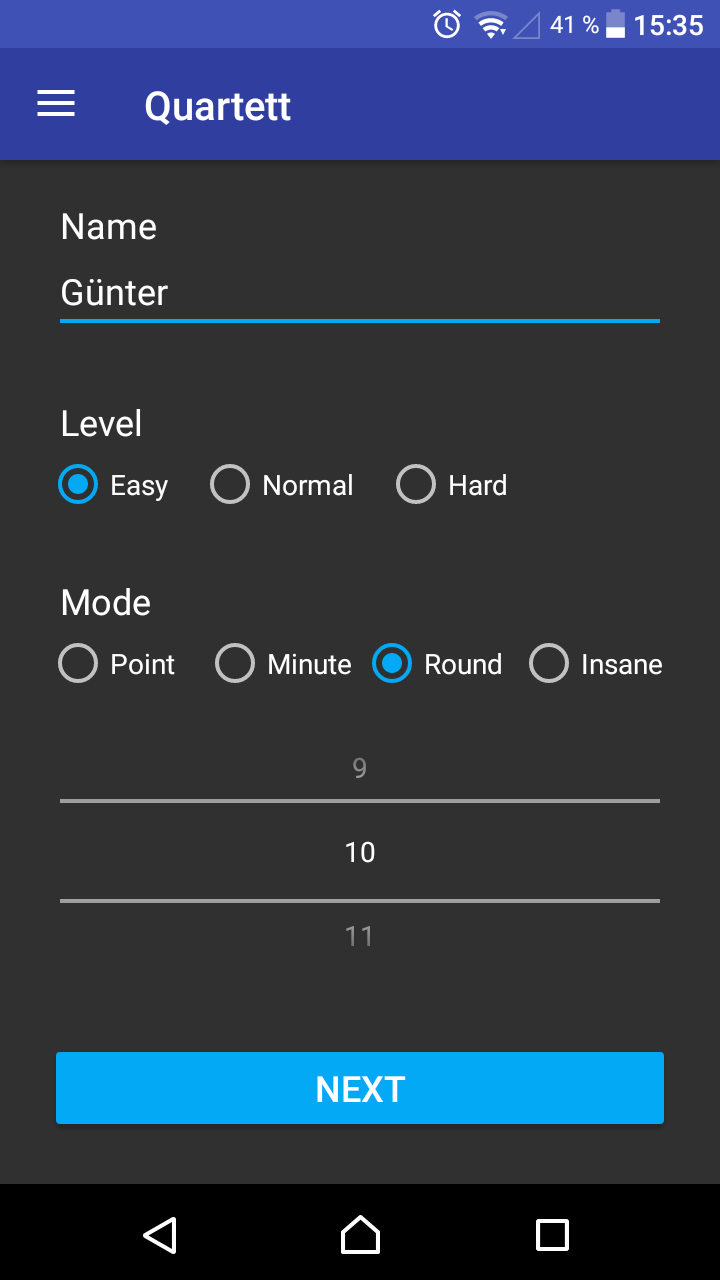
\includegraphics[width=4cm]{img/game_settings.png}
    \caption{Spieleinstellungen}
  \end{minipage}
  \hfill
  \begin{minipage}{0.45\textwidth}
    \centering
    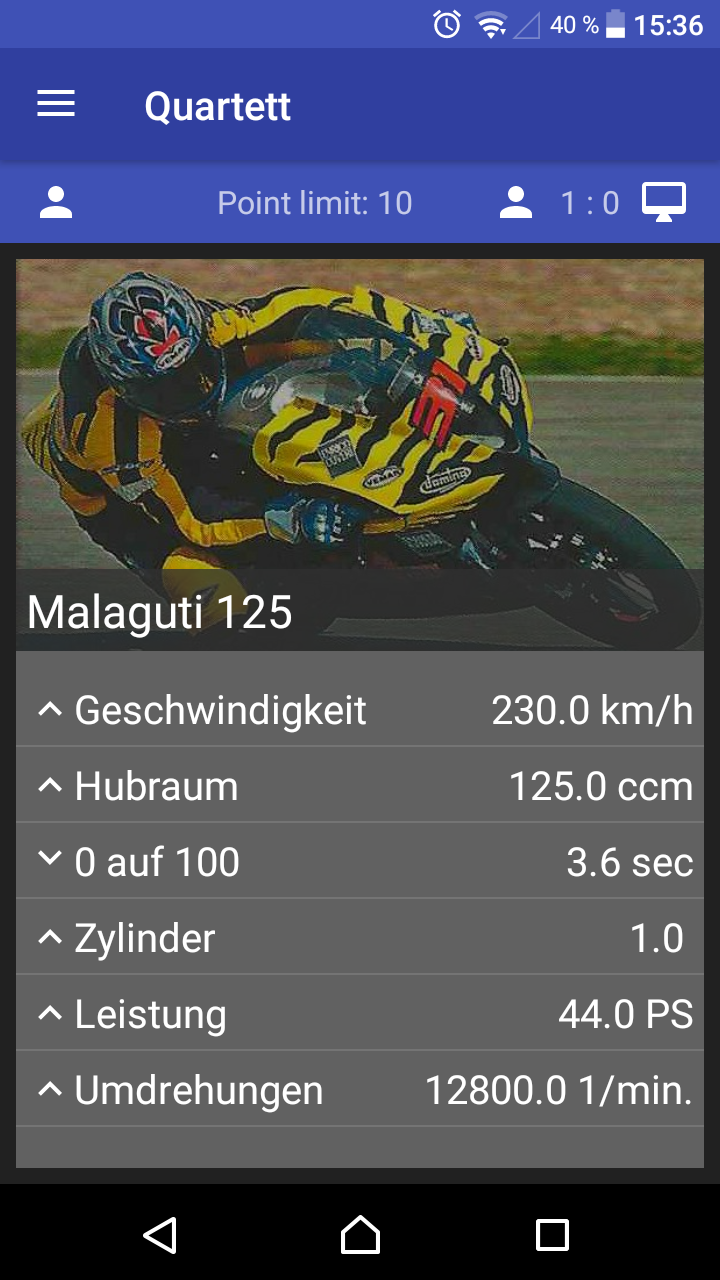
\includegraphics[width=4cm]{img/game_attributes.png}
    \caption{Attributauswahl}
  \end{minipage}
\end{figure}

\noindent
Im Einzelspielermodus der Quartett App werden vor jedem Spiel zunächst einige
Spieleinstellungen abgefragt. Der Name des Spielers wird für den Eintrag in die
lokale Rangliste verwendet. Außerdem kann der Schwierigkeitsgrad, also die
Stärke der KI, und der Spielmodus eingestellt werden. Um die Einstellungen nicht
bei jedem Spielstart erneut setzen zu müssen können Standardwerte für jeden
Parameter in den allgemeinen Spieleinstellungen hinterlegt werden. Nachdem alle
Einstellungen getroffen wurden wird der Spieler aufgefordert ein Deck
auszuwählen, mit welchem das Spiel gestartet werden soll. Dabei stehen nur Decks
zur Auswahl die bereits heruntergeladen worden sind. Nach der Auswahl eines
Decks startet das eigentliche Spiel. Dem Spieler wird eine Karte angezeigt, von
welcher ein Attribut ausgewählt werden kann. Dieses Attribut wird mit dem
Attribut verglichen, das die KI ausgewählt hat. Je nach Wert und Art des
Attributs gewinnt oder verliert der Spieler die Karte. Das Ergebnis des
Vergleichs wird in einer eigenen Ansicht präsentiert. Dort werden die beiden
Karten gegenüber gestellt und Gewinner (grün) und Verlierer (rot) entsprechend
eingefärbt. Hat der Spieler gewonnen so darf er erneut das Attribut bestimmen,
sonst wird der nächste Zug durch die KI ausgeführt. Ist schließlich die
Abbruchbedingung des Spiels erreicht (Zeit, Punkte, Runden) wird das Spiel
beendet und eine Punktezahl berechnet. War der Spieler besonders gut wird
außerdem automatisch ein Eintrag in der Rangliste vorgenommen. Danach besteht
die Möglichkeit das Spiel mit den selben Einstellungen erneut zu starten, die
Einstellungen zu ändern, oder in das Hauptmenü zurückzukehren.

\begin{figure}[!ht]
  \centering
  \begin{minipage}{0.45\textwidth}
    \centering
    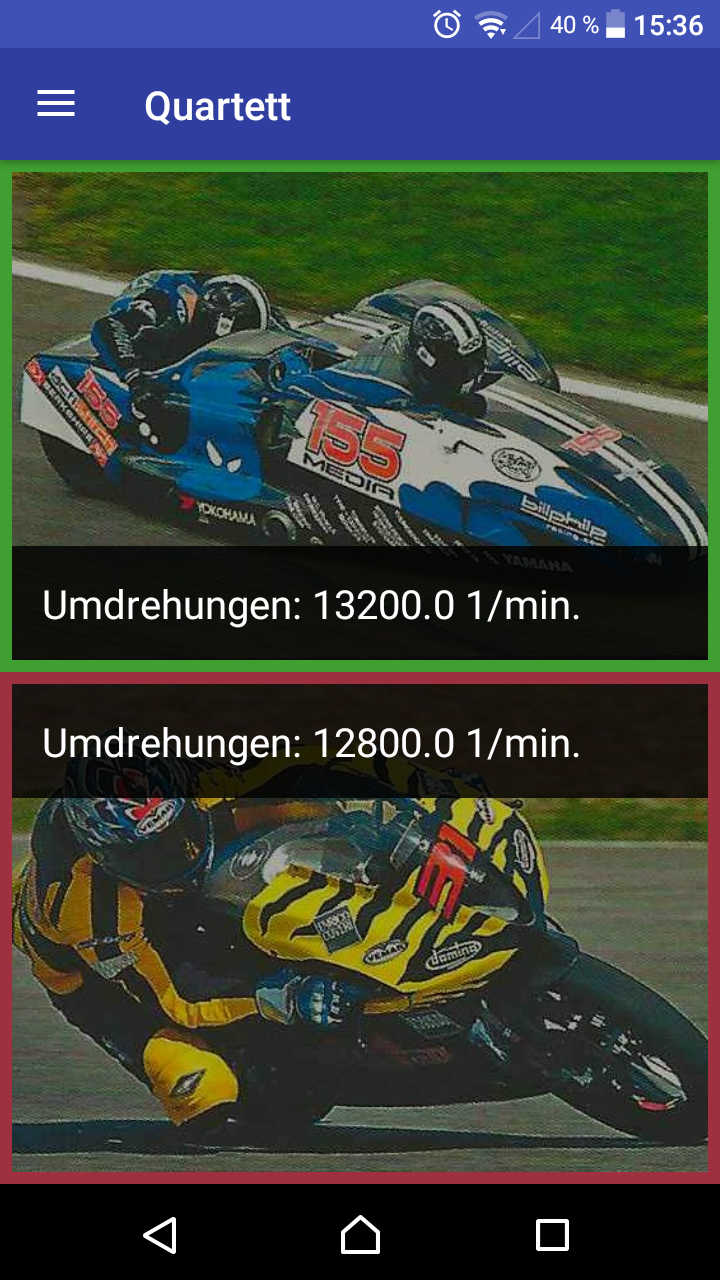
\includegraphics[width=4cm]{img/game_compare.png}
    \caption{Vergleichsansicht}
  \end{minipage}
  \hfill
  \begin{minipage}{0.45\textwidth}
    \centering
    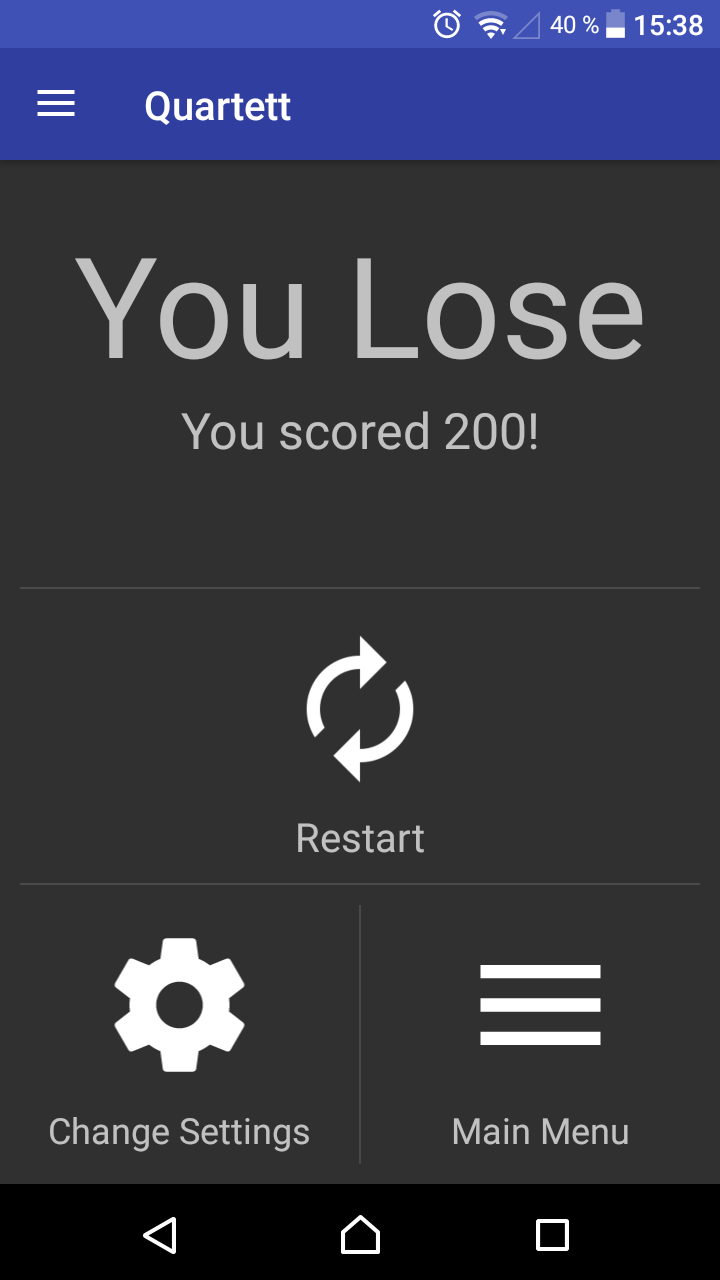
\includegraphics[width=4cm]{img/game_end.png}
    \caption{Spielende}
  \end{minipage}
\end{figure}

\noindent
Bei der Implementierung des Einzelspielers war besonders die KI eine
Herausforderung. Diese musste sich möglichst wie ein Spieler verhalten und kein
unfaires Spielerlebnis bieten, also nicht zu viel Wissen über den Spielstatus
erhalten. Die hier verwendete Implementierung erzeugt zunächst für jedes
Attribut eine nach eben diesem Attribut sortierte Liste der Karten. Danach wird
die Position der Karte in jeder dieser Listen ermittelt und dem jeweiligen
Attribut zugeordnet. Damit weiß die KI nun welches der Attribute das
\enquote{beste}, also das mit den höchsten Gewinnchancen ist. Je nach
eingestelltem Schwierigkeitsgrad wird die KI dann eher bessere oder eher
schlechtere Attribute auswählen. So wird ein Spieler simuliert, der das
Kartendeck, je nach Schwierigkeitsgrad, mehr oder weniger gut kennt, somit
abschätzen kann wie \enquote{gut} ein Attribut ist und auf Basis dieser
Schätzung seine Entscheidungen trifft. Außerdem erhält die KI mit dieser
Implementierung auch nicht mehr Informationen als ein menschlicher Spieler.
Unfaires Verhalten wird somit verhindert.

\subsubsection{Multiplayer}
Der Multiplayer bietet den Spielern die Möglichkeit über eine Internetverbindung gegeneinander zu spielen. Entscheidet sich der Nutzer zu einem Multiplayer Spiel gelangt dieser zu erst auf eine Activity die ihm eine Liste aller Spiele anzeigt die er gerade spielt und auch die Möglichkeit gibt ein neues Spiel zu starten. Wählt der Nutzer ein neues Spiel kann er sich entscheiden ob er automatisch einem anderen Spieler zugeteilt werden möchte oder gezielt mit einer bestimmten Person spielen möchte.

Im Mulitplayer modus wird im Gegensatz zum herkömmlichen Quartett immer abwechselnd gespielt egal wer die vorherige Runde gewonnen hat. Dies ist eine Designentscheidung die aus Usability Gründen getroffen wurde. Andernfalls könnte es vorkommen ein Spieler macht einen Zug, schließt die App um später weiter zu spielen aber in der Zwischenzeit gewinnt sein Gegner alle folgenden runden und beendet das Spiel ohne, dass der erste Spieler etwas mitbekommt.

Die technische Umsetzung wurde durch die bereits im Kapitel Libaries und Frameworks erwähnten Google Play Services extrem erleichtert. Durch die Verwendung dieser services mussten wir uns nur noch um den Client seitigen Teil der Anwendung kümmern. Hier war der anspruchsvollste Teil jedes mögliche Szenario abzudecken. Also entsprechend zu reagieren wenn einer der Spieler einen Zug gemacht hat und der andere zum Beispiel gerade noch das Ergebnis des vorherigen Zuges angeschaut hat oder gar nicht mehr innerhalb der App war. Da Quartett ein rundenbasiertes Spiel ist war die Synchronisation eher trivial.    
\subsection{Architektur}
\subsubsection{Datenmodell}

\begin{figure}[h]
  \centering
  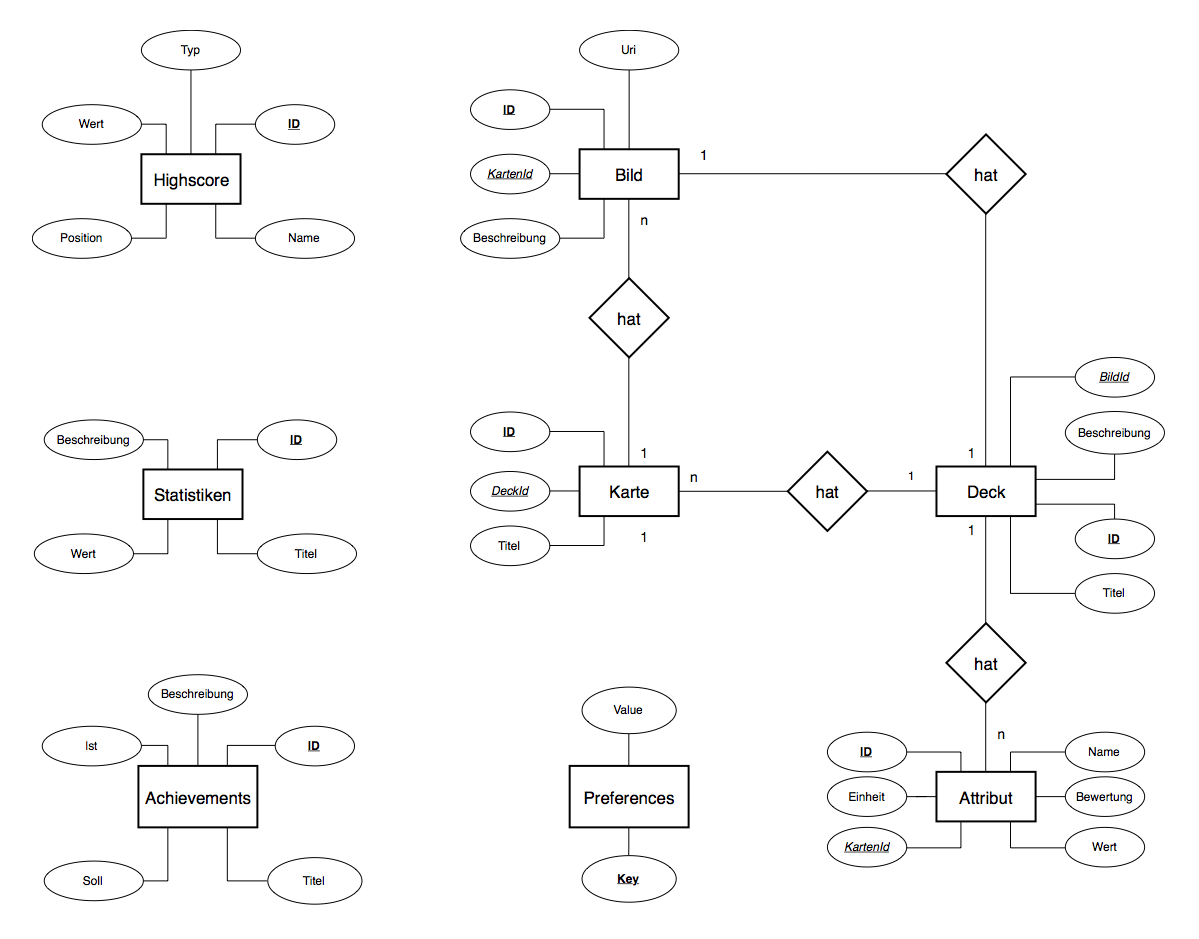
\includegraphics[width=\textwidth]{img/map_er.png}
  \caption{ER Diagramm des Datenmodells}
\end{figure}

\noindent
Im obigen ER Diagramm ist die Struktur unseres Datenmodells dargestellt. Zur
Realisierung wurde die in Android integrierte SQL Datenbank SQLite in
Kombination mit Sugar ORM verwendet. So konnten die einzelnen Entitäten direkt
über Klassen angesprochen werden und es mussten keine SQL Statements verwendet
werden. Allerdings beherrscht Sugar ORM in der verwendeten Version keine Listen
und Beziehungen zwischen den einzelnen Entitäten können mit Sugar ORM ebenfalls
nur schwierig oder gar nicht dargestellt werden. Die Daten der gespeicherten
Bilder wurden nicht in die SQL Datenbank geladen sondern direkt im internen
Speicher des Geräts abgelegt. Auch die \enquote{Preferences} werden nicht mit
SQL gespeichert sondern in den SharedPreferences des Android Systems abgelegt.
SharedPreferences ist eine einfach Key-Value Datenbank die sich kleine
Datenmengen eignet.

\subsubsection{Klassenstruktur}

\begin{figure}[!ht]
  \centering
  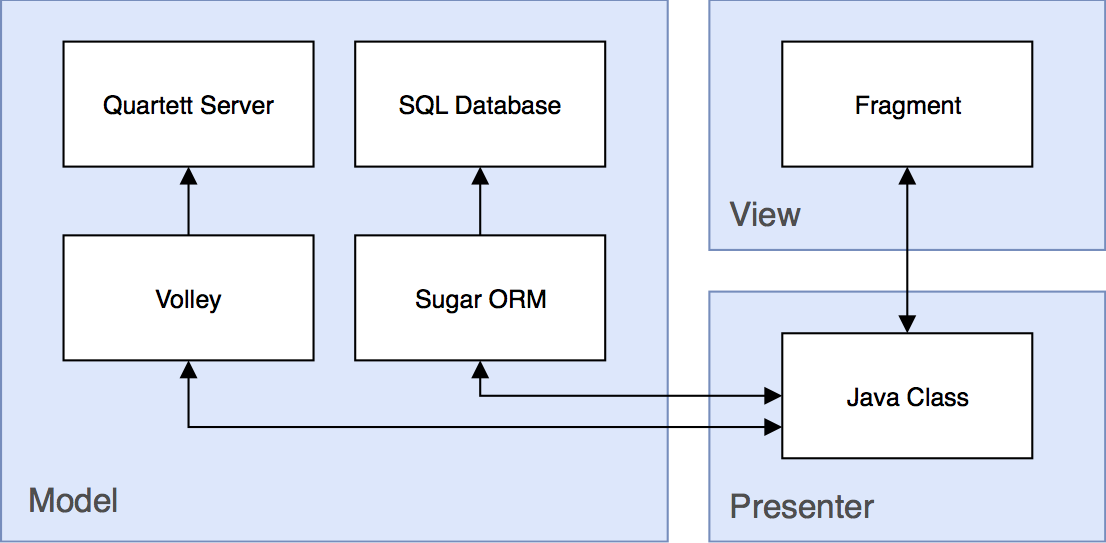
\includegraphics[width=\textwidth]{img/class_structure.png}
  \caption{Schematische Klassenstrukur der App mit MVP-Pattern}
\end{figure}

\noindent
Um die Applikation zu strukturieren wurde hier das Model-View-Presenter Pattern
angewendet. Mit diesem Pattern wird jede Activity in Model-, View- und
Presenter- Komponenten zerlegt. Die Model Komponenten beinhalten die
Zugriffsschicht auf die Datenbank mit allen zugehörigen Klassen. In der hier
vorgestellten App wird das Model durch Sugar ORM bzw. durch dessen
Entitätsklassen dargestellt. Außerdem wird die Serveranbindung, welche durch das
Volley Framework realisiert wird, ebenfalls zum Model gezählt. Es existiert
nur ein gemeinsames Model für alle Activities. Auf das Model kann nur vom
Presenter aus zugegriffen werden. Dieser verwaltet die
eigentlich Logik einer Activity. Dabei ist der Presenter selbst eine einfache
Java Klasse ohne direktes Wissen über das Android System oder die Datenbank.
Events der View werden an den Presenter weitergeleitet und dort bearbeitet. Der
Presenter kann zur Bearbeitung von Events sowohl auf das Model als auch auf die
View Komponenten zugreifen. Diese Komponenten beinhaltet die Anzeigeschicht und
verwaltet die einzelnen GUI-Elemente. In unserer App wird die View von einer
Fragment Klasse implementiert. Direkt kommuniziert die View nur mit dem
Presenter und greift nicht auf das Model zu. In der Praxis gibt es dabei
allerdings einige Ausnahmen.

\ \newline
Um z.B. das Anzeigen von Listen in Android effizient zu realisieren werden
sogenannte Adapter verwendet. Diese greifen meist direkt auf die Datenbank zu
und stellen die erhaltenen Daten direkt in einer ListView da. Damit können diese
Klassen nicht eindeutig den Model oder View Komponenten zugeordnet werden. Daher
implementieren diese meist sowohl die Eigenschaften des Models als auch der
View.

\ \newline
Durch die klare und immer gleichförmige Strukturierung in Model, View und
Presenter, wird das Erstellen von neuen Activities vereinfacht, da somit ein
klarer Arbeitsablauf gegeben ist. Auch das lesen und editieren von fremden Code
wird erleichtert, da von vornherein anhand der Benennung der einzelnen Klassen
klar ist welche Aufgaben diese Komponenten übernehmen.

\end{document}
